\section{Sudoku des équations}

\subsection{Sudoku numéro 1}
\begin{minipage}{0.55\textwidth}
    \begin{figure}[H]
        \center
        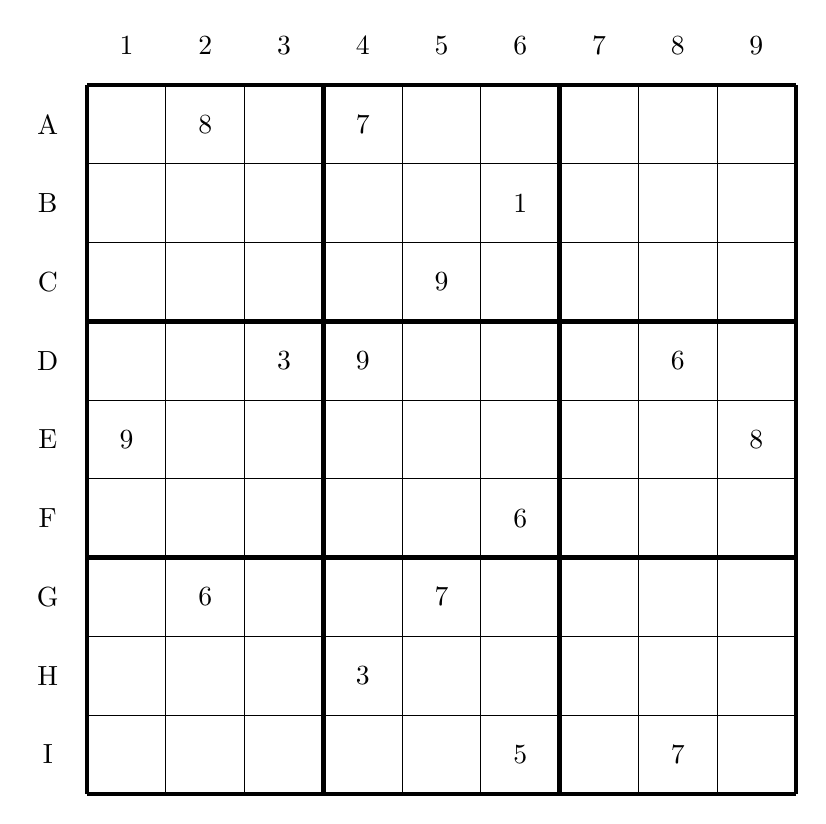
\begin{tikzpicture}[scale=1]
            \draw (0,0) grid (9,9);
            \draw[ultra thick,step=3] (0,0) grid (9,9);
            \foreach \x/\y in {1/A,2/B,3/C,4/D,5/E,6/F,7/G,8/H,9/I}
            {
                \draw node at (\x-0.5,9.5) {\x};
                \draw node at (-0.5,10-\x-0.5) {\y};
            }
                \draw node at (1.5,8.5) {8};
                \draw node at (3.5,8.5) {7};
                \draw node at (5.5,7.5) {1};
                \draw node at (4.5,6.5) {9};
                \draw node at (2.5,5.5) {3};
                \draw node at (7.5,5.5) {6};
                \draw node at (3.5,5.5) {9};
                \draw node at (0.5,4.5) {9};
                \draw node at (8.5,4.5) {8};
                \draw node at (
                    5.5,3.5) {6};
                \draw node at (1.5,2.5) {6};
                \draw node at (4.5,2.5) {7};
                \draw node at (3.5,1.5) {3};
                \draw node at (5.5,0.5) {5};
                \draw node at (7.5,0.5) {7};

        \end{tikzpicture}
\end{figure}
\end{minipage}
\hfil\vline\hfil
\begin{minipage}{0.40\textwidth}
Remplis les cases suivantes en résolvant les équations associées :
    \begin{multicols}{2}
        \begin{itemize}[leftmargin=1em]
            \item A3 : $x+5=9$
            \item B5 : $3x=18$
            \item B8 : $x-4=0$
            \item C4 : $4x=16$
            \item C8 : $8+x=13$
            \item C9 : $12-x=5$
            \item D2 : $x\div2=2$
            \item D7 : $9x=45$
            \item E5 : $x\div3=1$
            \item F2 : $4x+9=13$
            \item F3 : $3x-5=1$
            \item F7 : $2x-6=2$
            \item F8 : $12-3x=3$
            \item G1 : $2+x=3$
            \item G6 : $11x=99$
            \item H2 : $13x=26$
            \item H5 : $4x+2=6$
            \item I7 : $7-5x=2$
        \end{itemize}
    \end{multicols}

Case bonus si besoin :
        \begin{itemize}[leftmargin=1em]
            \item A7 : $2x-7=x+2$
            \item B7 : $5x-3=2x+3$
            \item C2 : $x\div3+2=x$
            \item D9 : $7x+2=5x+4$
            \item E6 : $2x+4=6x-12$
            \item G3 : $3(x+1)=2x+8$
            \item H8 : $2(x-5)=x-1$
            \item I1 : $4(2x+3)=6(x+3)$
        \end{itemize}
\end{minipage}


\subsection{Sudoku numéro 2}
\begin{minipage}{0.55\textwidth}
    \begin{figure}[H]
        \center
        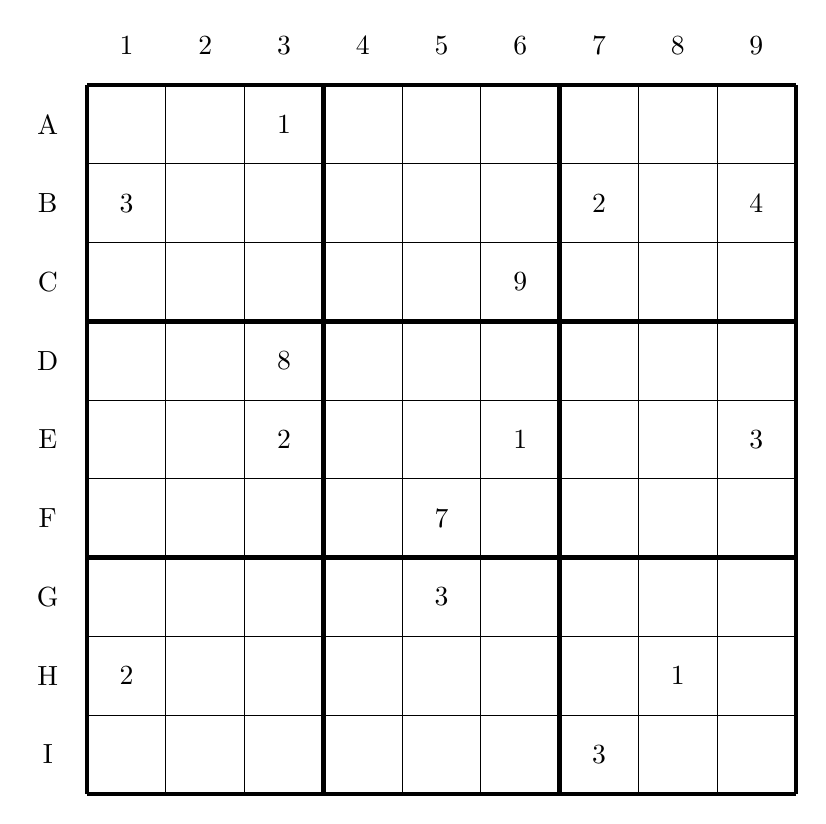
\begin{tikzpicture}[scale=1]
            \draw (0,0) grid (9,9);
            \draw[ultra thick,step=3] (0,0) grid (9,9);
            \foreach \x/\y in {1/A,2/B,3/C,4/D,5/E,6/F,7/G,8/H,9/I}
            {
                \draw node at (\x-0.5,9.5) {\x};
                \draw node at (-0.5,10-\x-0.5) {\y};
            }
                \draw node at (2.5,8.5) {1};
                \draw node at (0.5,7.5) {3};
                \draw node at (6.5,7.5) {2};
                \draw node at (8.5,7.5) {4};
                \draw node at (5.5,6.5) {9};
                \draw node at (2.5,5.5) {8};
                \draw node at (2.5,4.5) {2};
                \draw node at (5.5,4.5) {1};
                \draw node at (8.5,4.5) {3};
                \draw node at (4.5,3.5) {7};
                \draw node at (4.5,2.5) {3};
                \draw node at (0.5,1.5) {2};
                \draw node at (7.5,1.5) {1};
                \draw node at (6.5,0.5) {3};
        \end{tikzpicture}
\end{figure}
\end{minipage}
\hfil\vline\hfil
\begin{minipage}{0.40\textwidth}
Remplis les cases suivantes en résolvant les équations associées :
    \begin{multicols}{2}
        \begin{itemize}[leftmargin=1em]
            \item A2 : $3x=15$
            \item A6 : $4x=8$
            \item B2 : $x+3=10$
            \item B3 : $x+2=8$
            \item C5 : $x-3=5$
            \item C8 : $x-6=-1$
            \item D5 : $3x=6$
            \item E1 : $x+10=15$
            \item E4 : $x+3=7$
            \item E7 : $2x+3=21$
            \item F7 : $3x-6=-3$
            \item G2 : $7x-5x=2$
            \item G4 : $10x+6=26$
            \item H3 : $2x+4=18$
            \item H7 : $3x-2=10$
            \item H9 : $2x-4=3x-9$
            \item I4 : $3x-1=2x$
            \item I8 : $3x-3=2x+3$
        \end{itemize}
    \end{multicols}

Case bonus si besoin :
        \begin{itemize}[leftmargin=1em]
            \item A1 : $3x-7=2x+2$
            \item B8 : $4x-10=3x-1$
            \item D4 : $3(x+1)=2x+3\times4$
            \item F2 : $7x-3=5(x+3)$
            \item G9 : $2x+24=6x-12$
            \item H7 : $3(2x-8)=2x+12$
            \item I3 : $2(x-5)=x-1$
        \end{itemize}
\end{minipage}